%%This is a very basic article template.
%%There is just one section and two subsections.
\documentclass[a4paper, ngerman]{scrartcl}

\usepackage[T1]{fontenc}
\usepackage[utf8]{inputenc}
\usepackage[ngerman]{babel}
\usepackage{lmodern}
\usepackage{amsmath}
\usepackage{amsfonts}
\usepackage{hyperref}
\usepackage{graphicx}
\usepackage{paralist}
\usepackage[none]{hyphenat}

\sloppy



\hypersetup{ 
pdfborder = {0 0 0}, 
urlbordercolor = {0 0 0}, 
colorlinks = true,
linkcolor = black,
citecolor = black,
filecolor = black,
urlcolor  = black
}

\title{Software-Challenge 2016 \\ Twixt} 
\subtitle{Spielregeln}



%% Variablen
\newcommand{\FelderAnzahl}{\emph{576}}
\newcommand{\EmptyPlainPage}{\newpage\thispagestyle{plain}\ \newpage}
\newcommand{\RundenAnzahl}{\emph{30}}

\begin{document} 
\parindent0px
\maketitle

\begin{figure}[h!]
	\centering
	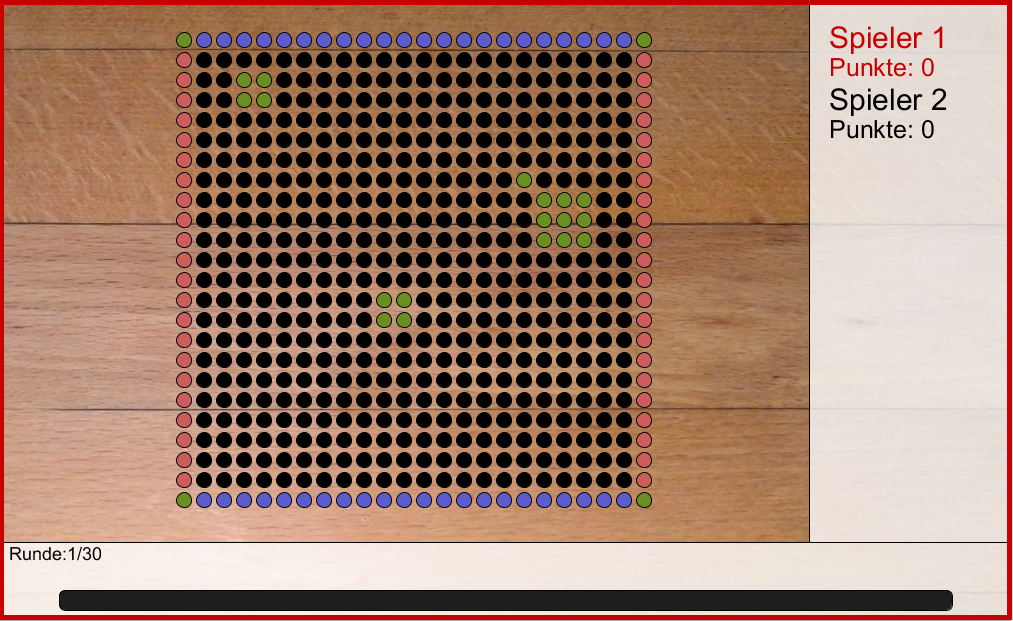
\includegraphics[width=\linewidth]{bilder/gui.png} 
\end{figure}
\vspace*{\fill}
"Die Nutzung des Spielkonzeptes "twixt" (Name, Spielregeln
und Grafik) erfolgt mit freundlicher Genehmigung des Kosmos Verlags."
\newpage
\tableofcontents
\newpage

\section{Einführung}
In dieser Anleitung werden die Elemente und Regeln des Spiels \emph{Twxit} der
Software-Challenge 2016 erläutert.\\
Bei Twixt versuchen zwei Spieler durch abwechselndes setzen von Strommasten eine
durchgehende Verbindung zwischen den beiden gegenüberliegenden Spielfeldrändern
herzustellen, und gleichzeitig den Gegenspieler daran zu hindern, das Gleiche zu
tun. 

\section{Das Spielbrett}
Das Spielbrett setzt sich aus 576 Bauflächen für Strommasten zusammen, die
anfangs noch nicht besetzt sind.
Diese Bauplätze gehören entweder schon zu einer Farbe, sind von Sumpf bedeckt
(sind also nicht bebaubar) oder sind keines von beiden.
Anfangs werden zufällig Sumpfelder generiert, wobei es sich um einen kleinen
Sumpf (1x1), zwei mittlere Sümpfe (2x2) und einen großen Sumpf (3x3) handelt,
die sich auch überschneiden dürfen. Spielbrett ist in den Abbildungen 1-3 zu
sehen.

\begin{figure}[h!]
		\centering
		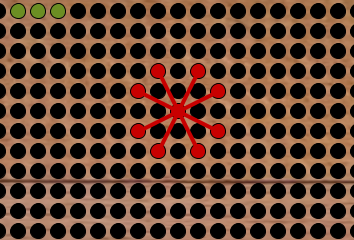
\includegraphics[scale = 0.8]{bilder/setzzug.png}
		\caption{Alle möglichen Leitungen}
		\label{fig:Leitungen}
\end{figure}
	
\section{Spielablauf}	 
Zu Beginn des Spiels setzt zunächst Rot einen neuen Strommast auf ein
freies Feld, also ein Feld, das weder ein Sumpffeld noch ein Feld der
gegnerischen Farbe ist und auf dem sich noch kein Strommast befindet. Danach tut Blau dasselbe, während beide versuchen
ihre beiden Farbzonen (farbig markierte Felder; für Rot sind diese links und
rechts, für Blau  oben und unten) mit einer zusammenhängenden Leitung zu
verbinden.
	%% an Beispiel erklären
	Bei einem Zug ist es möglich, dass sich dadurch eine oder mehrere
	neue Leitungen bilden. Eine neue Leitung bildet sich, wenn sich ein eigener
	Strommast in folgendem Abstand zu dem gesetztem Strommast befindet: Zwei
	waagerecht und ein Feld senkrecht oder eins waagerecht und zwei Felder
	senkrecht. Dies geschieht aber nur, wenn bisher keine Leitung existiert, die
	die entstehende Leitung kreuzen würde.
	Ein Beispiel, welche Leitungen von einem Strommast aus möglich sind, ist
	in Abbildung 1 zu sehen.
	 
	
\section{Ende des Spiels} 
	Das Spiel endet, sobald es einer der Spieler geschafft hat, seine beiden
	Farbzonen mit einer zusammenhängenden Leitung zu verbinden, spätestens jedoch
	nach 30 Runden.
	Für die Berechnung der Punkte von Rot ist allein diejenige zusammenhängende
	Leitung von Rot entscheidend, welche in horizontaler Richtung die längste Ausdehnung
	hat. Die Ausdehnung dieser Leitung in horizontaler Richtung ergibt die Punktezahl
	für Rot. Entsprechend zählt für Blau die vertikale Ausdehnung.
	In dem in Abbildung 2 gezeigten Beispiel erhält Rot deshalb 4 Punkte
	(die kürzere Leitung zählt nicht) und Blau 8 (es zählt ausschließlich
	die vertikale Richtung). Das Spiel gewinnt derjenige Spieler, der am Spielende die
	meisten Punkte hat.
	Ist die so ermittelte Punktzahl gleich, ist das Ergebnis unentschieden.
\section{Die graphische Benutzeroberfläche}

\subsection{Graphische Benutzeroberfläche}

	 
	In Abbildung~\ref{fig:GUI} ist ein Überblick der graphischen Benutzeroberfläche
	zu sehen. Die markanten Spielelemente sind mit \emph{A-C} gekennzeichnet.
	\begin{figure}[H]
		\centering		
		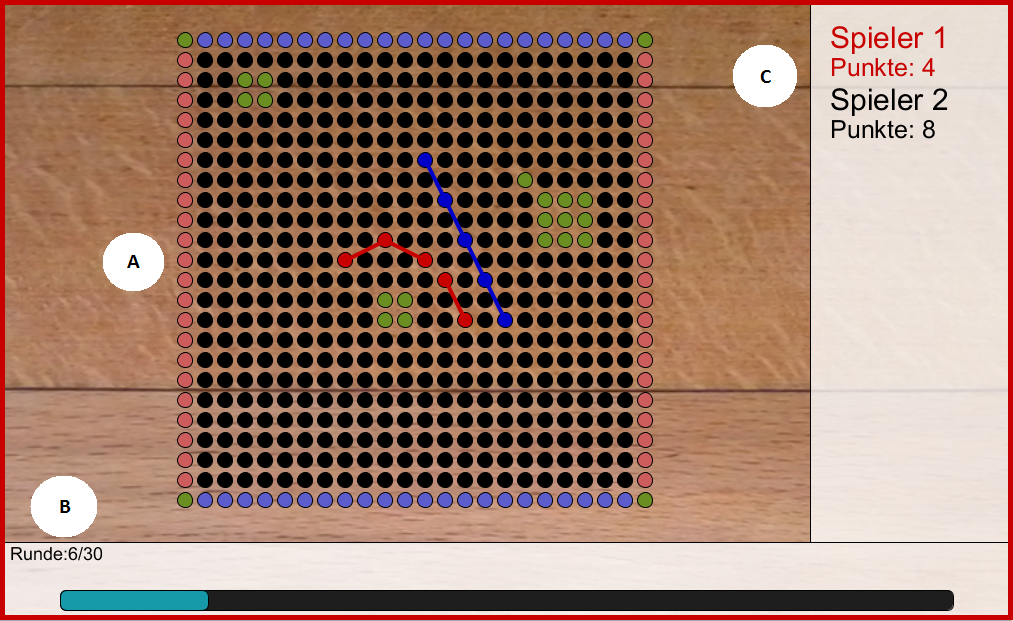
\includegraphics[scale = 0.6]{bilder/uebersicht.png} 
		\caption{Überblick der GUI}
		\label{fig:GUI}
	\end{figure}
	 
	%% wie ist die Benutzeroberfläche?
\begin{compactenum}[A)] 
\item Das Spielbrett
\item Die Spielfortschrittsanzeige  
\item Die Punktestand der Spieler
	\end{compactenum}
	
\subsection{Das Einstellungsmenü} 
	 \begin{figure}[H]
		\centering
		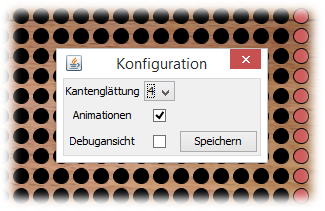
\includegraphics[scale=0.6]{bilder/konfiguration.png}
		\caption{Das Einstellungsmenü}
		\label{fig:Configuration}
	\end{figure}
	
	Ein Einstellungsmenü mit Darstellungsoptionen wird in Abbildung 3 dargestellt
	und lässt sich über die Taste 'C' anzeigen. Dazu muss das
Spielfeld den Tastaturfokus haben (erforderlichenfalls
vorher Mausklick auf das Spielfeld). Es stehen dort
folgende Einstellungen zur Verfügung: 

\textbf{Kantenglättung} verbessert die Optik des
Spiels, ist aber rechenintensiv, diese hat Einstellungen von 0 bis 8 und ist
standardmäßig auf 4 gestellt.
Auf sehr langsamen Rechnern sollte sie daher auf 0 gestellt werden.
\textbf{Animationen} gibt es hier nicht.\\
Die \textbf{Debugansicht} zeigt Debug-Hilfestellungen zu einzelnen Zügen und
die Framerate an.
Diese Hilfestellungen sind Texte, die ein Spielclient einem Zug beifügen kann, den er
an den Spielserver sendet.
	
\end{document}
